\section{391 --- Perfect Rectangle}
\definecolor{lhg}{RGB}{164,165,165}
Given $N$ axis-aligned rectangles where $N > 0$, determine if they all together form an exact cover of a rectangular region.
\par
Each rectangle is represented as a bottom-left point and a top-right point. For example, a unit square is represented as $[1,1,2,2]$. (coordinate of bottom-left point is $(1, 1)$ and top-right point is $(2, 2)$).

\paragraph{Example 1:}
\begin{flushleft}
\textbf{Input}:
\begin{table}[H]
\begin{tabular}{cccc}
1 & 1 & 3 & 3\\
3 & 1 & 4 & 2\\
3 & 2 & 4 & 4\\
1 & 3 & 2 & 4\\
2 & 3 & 3 & 4
\end{tabular}
\end{table}
\textbf{Output}: \texttt{true}
\\
\textbf{Explanation}: All 5 rectangles together form an exact cover of a rectangular region.


\begin{figure}[H]
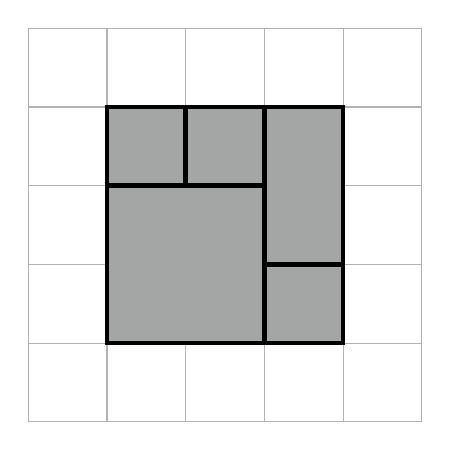
\begin{tikzpicture}
\draw[gray!60!, thin] (0,0) grid(5,5);
\draw[fill=lhg, ultra thick] (1,1) rectangle ++(2,2);
\draw[fill=lhg, ultra thick] (1,3) rectangle ++(1,1);
\draw[fill=lhg, ultra thick] (2,3) rectangle ++(1,1);
\draw[fill=lhg, ultra thick] (3,1) rectangle ++(1,1);
\draw[fill=lhg, ultra thick] (3,2) rectangle ++(1,2);
\end{tikzpicture}
\end{figure}

\end{flushleft}

\paragraph{Example 2:}
\begin{flushleft}
\textbf{Input}:
\begin{table}[H]
\begin{tabular}{cccc}
1 & 1 & 2 & 3 \\
1 & 3 & 2 & 4\\
3 & 1 & 4 & 2 \\
3 & 2 & 4 & 4
\end{tabular}
\end{table}
\textbf{Output}: \texttt{false}
\\
\textbf{Explanation}: There is a gap between the two rectangular regions.
\begin{figure}[H]
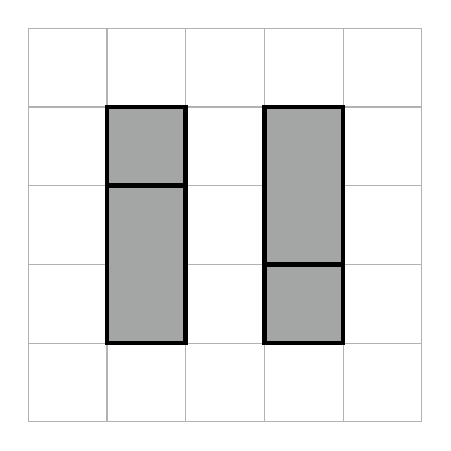
\begin{tikzpicture}
\draw[gray!60!, thin] (0,0) grid(5,5);
\draw[fill=lhg, ultra thick] (1,1) rectangle ++(1,2);
\draw[fill=lhg, ultra thick] (1,3) rectangle ++(1,1);
\draw[fill=lhg, ultra thick] (3,1) rectangle ++(1,1);
\draw[fill=lhg, ultra thick] (3,2) rectangle ++(1,2);
\end{tikzpicture}
\end{figure}
\end{flushleft}


\paragraph{Example 3:}
\begin{flushleft}
\textbf{Input}:
\begin{table}[H]
\begin{tabular}{cccc}
1 & 1 & 3 & 3\\
3 & 1 & 4 & 2\\
1 & 3 & 2 & 4\\
3 & 2 & 4 & 4
\end{tabular}
\end{table}
\textbf{Output}: \texttt{false}
\\
\textbf{Explanation}: Because there is a gap in the top center.
\begin{figure}[H]
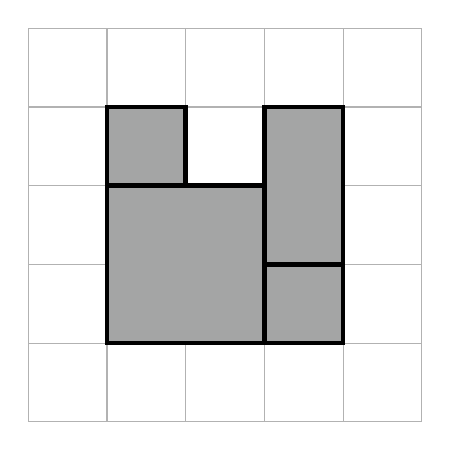
\begin{tikzpicture}
\draw[gray!60!, thin] (0,0) grid(5,5);
\draw[fill=lhg, ultra thick] (1,1) rectangle ++(2,2);
\draw[fill=lhg, ultra thick] (1,3) rectangle ++(1,1);
\draw[fill=lhg, ultra thick] (3,1) rectangle ++(1,1);
\draw[fill=lhg, ultra thick] (3,2) rectangle ++(1,2);
\end{tikzpicture}
\end{figure}
\end{flushleft}

\paragraph{Example 4:}
\begin{flushleft}
\textbf{Input}:
\begin{table}[H]
\begin{tabular}{cccc}
1 & 1 & 3 & 3\\
3 & 1 & 4 & 2\\
1 & 3 & 2 & 4\\
2 & 2 & 4 & 4
\end{tabular}
\end{table}
\textbf{Output}: \texttt{false}
\\
\textbf{Explanation}: Because two of the rectangles overlap with each other.
\begin{figure}[H]
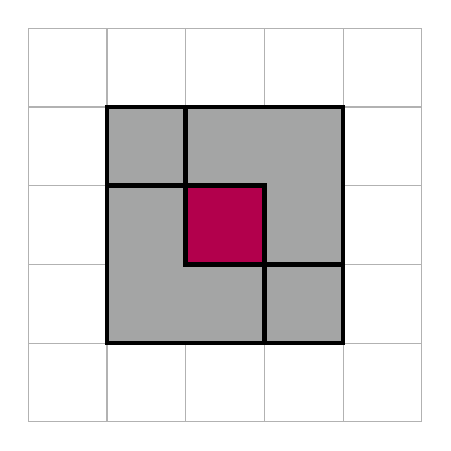
\begin{tikzpicture}
\draw[gray!60!, thin] (0,0) grid(5,5);
\draw[fill=lhg, ultra thick] (1,1) rectangle (3,3);
\draw[fill=lhg, ultra thick] (3,1) rectangle (4,2);
\draw[fill=lhg, ultra thick] (1,3) rectangle (2,4);
\draw[fill=lhg, ultra thick] (2,2) rectangle (4,4);
\draw[fill=red!70!blue!, ultra thick] (2,2) rectangle ++(1,1);
\end{tikzpicture}
\end{figure}
\end{flushleft}

\subsection{Coordinate Compression}
This approach will cause LTE.

\setcounter{lstlisting}{0}
\begin{lstlisting}[style=customc, caption={Coordinate Compression}]
bool isRectangleCover( vector<vector<int>>& rectangles )
{
    if( rectangles.empty() )
    {
        return false;
    }

    map<int, int> m;

    //compress the coordinates
    for( const auto& rect :  rectangles )
    {
        for( int n :  rect )
        {
            auto it = m.find( n );
            if( it == m.end() )
            {
                m.emplace( n, 0 );
            }
        }
    }

    int rank = 0;

    //get the rank for each number
    for( auto& p : m )
    {
        p.second = rank;
        ++rank;
    }

    int min_x = INT_MAX;
    int max_x = INT_MIN;
    int min_y = INT_MAX;
    int max_y = INT_MIN;

    //reset the coordinates of the rectangles
    //to the compressed values
    for( auto& rect : rectangles )
    {
        rect[0] = m[rect[0]];
        rect[1] = m[rect[1]];
        rect[2] = m[rect[2]];
        rect[3] = m[rect[3]];

        min_x = ( min )( min_x, rect[1] );
        min_y = ( min )( min_y, rect[0] );
        max_x = ( max )( max_x, rect[3] );
        max_y = ( max )( max_y, rect[2] );
    }

    vector<vector<unsigned char>> v_cover( max_x, vector<unsigned char>( max_y, 0 ) );

    //iterate each compressed rectangle
    //check if any overlap exists
    //and then mark each unit rectangle as covered
    for( const auto& rect : rectangles )
    {
        for( int x = rect[1]; x < rect[3]; ++x )
        {
            for( int y = rect[0]; y < rect[2]; ++y )
            {
                if( v_cover[x][y] == 1 )
                {
                    return false;
                }

                v_cover[x][y] = 1;
            }
        }
    }

    //for each unit rectangle, check if it is covered
    for( int x = min_x; x < max_x; ++x )
    {
        for( int y = min_y; y < max_y; ++y )
        {
            if( v_cover[x][y] == 0 )
            {
                return false;
            }

        }
    }

    return true;
}
\end{lstlisting}

\subsection{Count Vertices}
There are three kinds of vertices for each rectangle: 
\begin{enumerate}
\item The corner of the rectangle that is formed from all inputs: This kind of vertices can only appear only once for all inputs. Otherwise, there must be overlap.
\begin{figure}[H]
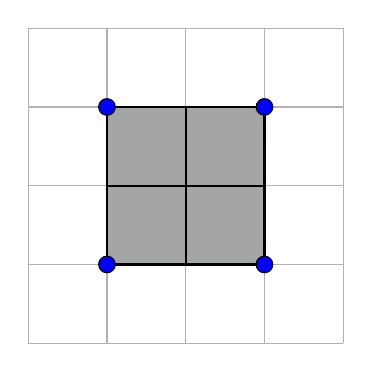
\begin{tikzpicture}
\draw[gray!60!, thin] (0,0) grid (4,4);
\draw[fill=lhg, thick] (1,1) rectangle ++(1,1);
\draw[fill=lhg, thick] (2,1) rectangle ++(1,1);
\draw[fill=lhg, thick] (1,2) rectangle ++(1,1);
\draw[fill=lhg, thick] (2,2) rectangle ++(1,1);
\draw[fill=blue] (1,1) circle (3pt);
\draw[fill=blue] (3,1) circle (3pt);
\draw[fill=blue] (1,3) circle (3pt);
\draw[fill=blue] (3,3) circle (3pt);
\end{tikzpicture}
\end{figure}
\item 两个矩形并排相邻所重合的顶点
\begin{figure}[H]
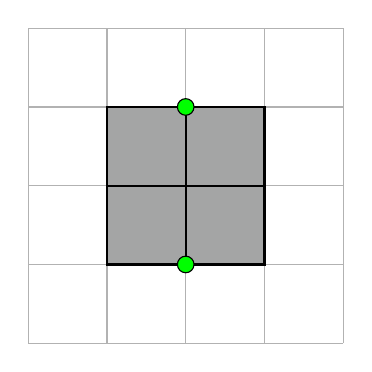
\begin{tikzpicture}
\draw[gray!60!, thin] (0,0) grid (4,4);
\draw[fill=lhg, thick] (1,1) rectangle ++(1,1);
\draw[fill=lhg, thick] (2,1) rectangle ++(1,1);
\draw[fill=lhg, thick] (1,2) rectangle ++(1,1);
\draw[fill=lhg, thick] (2,2) rectangle ++(1,1);
\draw[fill=green] (2,1) circle (3pt);
\draw[fill=green] (2,3) circle (3pt);
\end{tikzpicture}
\end{figure}
\item 四个矩形相邻所重合的顶点
\begin{figure}[H]
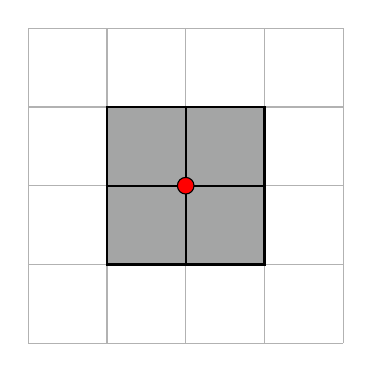
\begin{tikzpicture}
\draw[gray!60!, thin] (0,0) grid (4,4);
\draw[fill=lhg, thick] (1,1) rectangle ++(1,1);
\draw[fill=lhg, thick] (2,1) rectangle ++(1,1);
\draw[fill=lhg, thick] (1,2) rectangle ++(1,1);
\draw[fill=lhg, thick] (2,2) rectangle ++(1,1);
\draw[fill=red] (2,2) circle (3pt);
\end{tikzpicture}
\end{figure}
\end{enumerate}
可以看出,每个绿点其实都是两个顶点的重合,每个红点都是四个顶点的重合,而每个蓝点只有一个顶点,因此,用一个hash set,来记录遇到的vertices,如果vertices在set中,就将其删除,否则将其加入到set中,由于绿点和红点都是偶数,所以最终在set中只会留下蓝点的坐标。因此在最后只需要检查在set中是否还有4个顶点坐标存在,以及所有矩形的面积之和和这四个蓝点坐标构成的矩形面积是否相等。
\par
为了能够将顶点坐标放入hash set中,这里采用一个小技巧,将坐标的数字转换成字符串并在两个数字之间用一个特殊的字符拼接起来,比如井号,例如坐标(2,3),就转换成2\#3

\begin{lstlisting}[style=customc, caption={Count Vertices}]
bool isRectangleCover( vector<vector<int>>& rectangles )
{
    if( rectangles.empty() )
    {
        return false;
    }

    unordered_set<string> verts;

    int x_min = INT_MAX;
    int x_max = INT_MIN;
    int y_min = INT_MAX;
    int y_max = INT_MIN;

    int total_area = 0;

    for( auto& rect : rectangles )
    {
        x_min = ( min )( x_min, rect[1] );
        y_min = ( min )( y_min, rect[0] );
        x_max = ( max )( x_max, rect[3] );
        y_max = ( max )( y_max, rect[2] );

        total_area += ( rect[3] - rect[1] ) * ( rect[2] - rect[0] );

        string bl = to_string( rect[0] ) + '#' + to_string( rect[1] );
        string tr = to_string( rect[2] ) + '#' + to_string( rect[3] );
        string br = to_string( rect[0] ) + '#' + to_string( rect[3] );
        string tl = to_string( rect[2] ) + '#' + to_string( rect[1] );

        //bottom-left
        auto it = verts.find( bl );
        if( it == verts.end() )
        {
            verts.emplace( bl );
        }
        else
        {
            verts.erase( bl );
        }

        //top-right
        it = verts.find( tr );

        if( it == verts.end() )
        {
            verts.emplace( tr );
        }
        else
        {
            verts.erase( tr );
        }

        //top-left
        it = verts.find( tl );

        if( it == verts.end() )
        {
            verts.emplace( tl );
        }
        else
        {
            verts.erase( tl );
        }

        //bottom-right
        it = verts.find( br );

        if( it == verts.end() )
        {
            verts.emplace( br );
        }
        else
        {
            verts.erase( br );
        }
    }


    if( verts.size() != 4 )
    {
        return false;
    }

    //we need to put y first and x second
    //to conform the way we form the string when
    //iterating the rectangles
    auto bl = to_string( y_min ) + '#' + to_string( x_min );
    auto tl = to_string( y_max ) + '#' + to_string( x_min );
    auto br = to_string( y_min ) + '#' + to_string( x_max );
    auto tr = to_string( y_min ) + '#' + to_string( x_max );

    if( verts.find( bl ) == verts.end() )
    {
        return false;
    }
    if( verts.find( tr ) == verts.end() )
    {
        return false;
    }
    if( verts.find( br ) == verts.end() )
    {
        return false;
    }
    if( verts.find( tl ) == verts.end() )
    {
        return false;
    }

    //check if the areas are equal
    return total_area == ( x_max - x_min ) * ( y_max - y_min );
}
\end{lstlisting}